\chapter{The Newton-Raphson Method}
\section{Introduction: Root-Finding Methods}

Objective: To Find the location of \emph{roots} of a function.

\marginnote{* \textbf{A Root} of a function is a value $x$ at which $f(x)=0$, or the $x$ values at which the graph of $f$ intersects the $x$-axis ($x$-intercepts).}

\begin{examplebox}{Find the roots of the following functions.}

a) $f(x) = 5-3x$

\vspace{1cm}

b) $f(x) = 2x^2 +x -1$

\vspace{1cm}

\end{examplebox}

Now what about roots of $f(x) = x^3 -5x +1$?

\marginnote{
	* The discriminant of the general cubic equation $ax^{3 }+bx^{2 }+cx+d = 0, a\neq0$ exists and can be written as
	\[
	\frac{4(b^{2}-3ac)^{3}-(2b^{3}-9abc+27a^{2}d)^{2}}{27a^{2}}.
	\]
	But the solution for $x $ can be complecated. Hence, we introduce the \emph{Newton-Raphson Method}.
}

\begin{mybox}{Newton-Raphson Method}
Newton-Raphson Method is a numerical analysis technique for finding a root of a function.

It involves finding successive tangent lines to the graph of $f$, following a certain algorithm until we get close enough to the root.
\end{mybox}


\section{Derive the iteration formula}

A function $f$ is given and assume $r$ is a root of $f$ that we wish to approximate, we also assume $f$ is differentiable in an interval containing $r$.

Suppose an initial approximation of $r$ is also given, call that $x_0$.\\

$\rightsquigarrow$ \textbf{Algorithm}:

1) Draw a tangent line to the curve of $f$ at the point $(x_0, f(x_0))$:

\marginnote{(What is the equation of this tangent line at $(x_0, f(x_0))$?)}

\vspace{3cm}

2) Continue the tangent line such that it intersects the $x$-axis at a point, call that point $x_1$. $x_1$ is our new approximation:

\marginnote{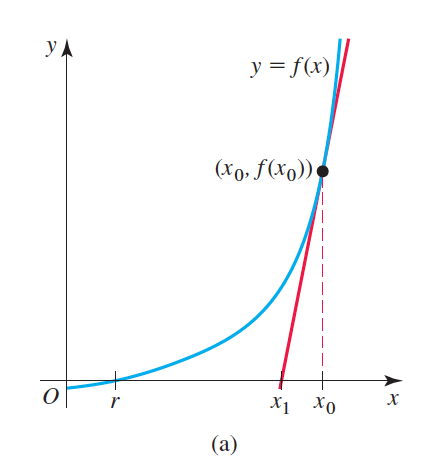
\includegraphics[scale=0.8]{pics/new1}}

\vspace{1cm}
\[
	x_{1} = \qquad \qquad \qquad \qquad
\]
\vspace{1cm}

3) Now repeat steps 1 and 2 for $x_1$:

\marginnote{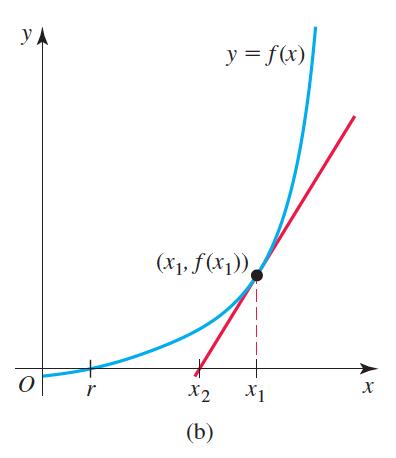
\includegraphics[scale=0.8]{pics/new2}}

 Draw a tangent line to the curve of $f$ at the point $(x_1, f(x_1))$, continue the tangent line such that it intersects the $x$-axis at $x_2$ and repeat the steps.

\vspace{3cm}
\[
	x_{2} = \qquad \qquad \qquad \qquad
\]
\vspace{1cm}

 Repeating the algorithm for each point, we will obtain a sequence of points, $\{x_0, x_1, x_2, x_3, ...\}$, that ideally get closer and closer to the root $r$.

\marginnote{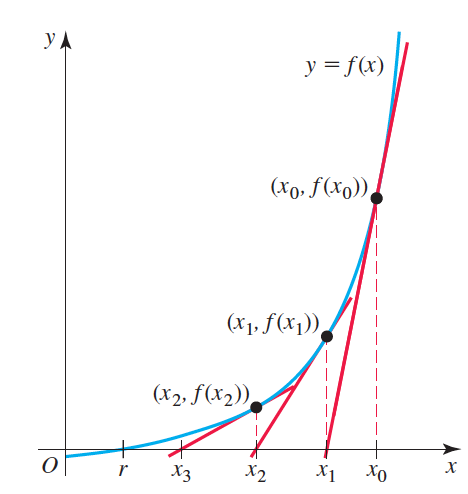
\includegraphics[scale=0.8]{pics/new4}}

\vspace{2cm}
\[
	x_{3} = \qquad \qquad \qquad \qquad
\]
\vspace{1cm}

This pattern continues: If a previous approximation is known, say $x_n$, then the new approximation is calculated by the following formula:

\begin{equation}
	x_{n+1 } = \qquad \qquad \qquad \qquad
	\label{eq:iteration}
\end{equation}


\begin{examplebox}{Find the root of cubic equation}
Find the root of $f(x) = x^{3}-5x+1 = 0 $ with inital approximations $x_{0 } = -3, x_{0 } = 1 $ and $x_{0 }=4 $ with two steps.
\end{examplebox}
\marginnote{
	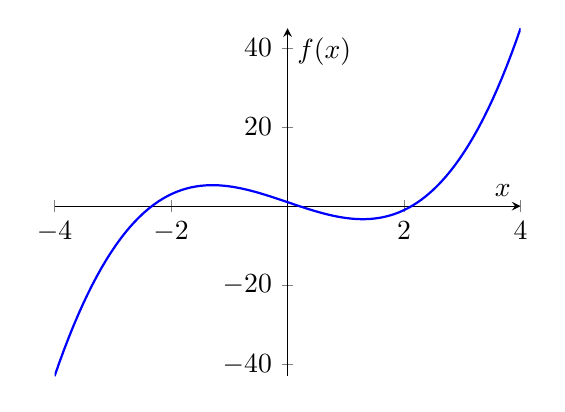
\begin{tikzpicture}
    \begin{axis}[
        axis lines = middle,
        xlabel = \(x\),
        ylabel = {\(f(x)\)},
        domain=-4:4,
        samples=100,
        width=7.5cm,
        height=6cm,
        ymajorgrids=false,
        xmajorgrids=false,
    ]
    \addplot [
        thick,
        blue,
    ] {x^3 - 5*x + 1};
    \end{axis}
\end{tikzpicture}
}

\begin{align*}
	f(x) &= x^{3}-5x+1\\
			 &\\
	f'(x) &=\\
			 &\\
	x_{n+1} &=
\end{align*}

\newpage
\marginnote{
\noindent
\textbf{Remark 1.} Newton's method is an example of a repetitive loop calculation called an \textit{iteration}. It is mainly done by calculators and computers and it is included in many scientific computing software.\\

\textbf{Remark 2.} When to stop?

They are different way to decide when to terminate the iterations. Either the number of iterations are given, or the number of agreeing digits between two successive approximations are given, for instance continue the iterations until two successive approximations agree to 4 digits. The effectiveness of the algorithm is to get close enough to the root (small error) as quickly as possible (not many iterations).
}
\begin{center}
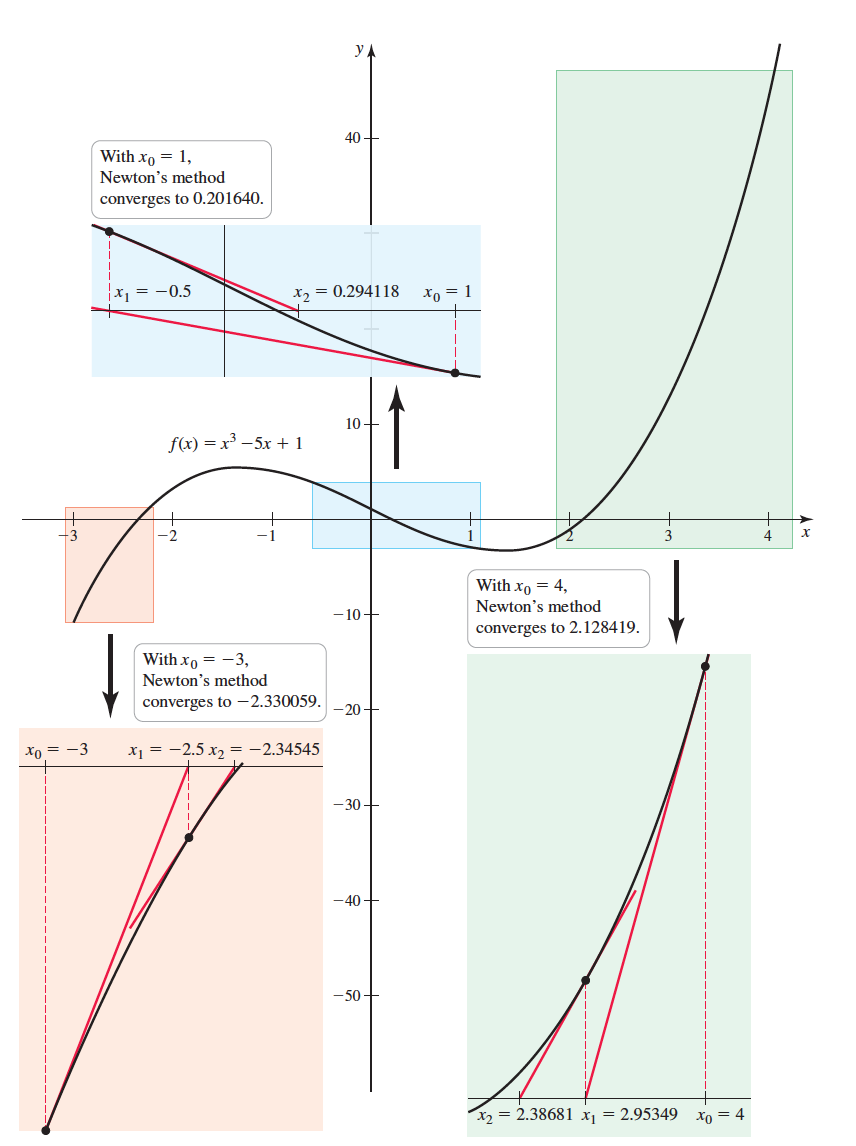
\includegraphics[scale=1]{pics/Newton2}
\end{center}

\begin{examplebox}{}
Use Newton's method to estimate the value for $\sqrt{10}$.
Stop calculating approximations when two successive approximations agree to four digits to the right of the decimal point.
\end{examplebox}

\newpage

\marginnote{
\textbf{Remark 3.} Newton's method is not always working. The location of the initial approximation is important.

\vspace{1cm}
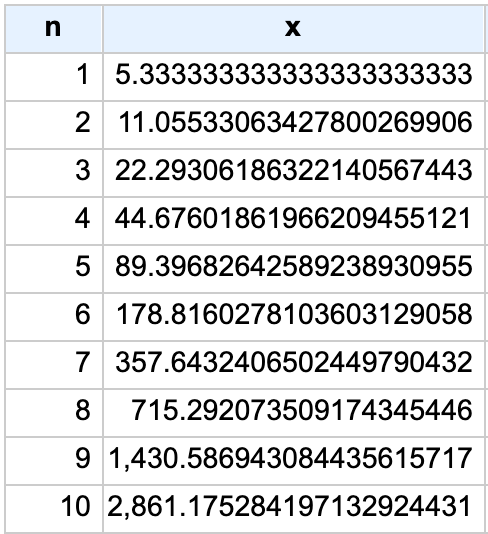
\includegraphics[scale=0.8]{pics/new6}
}
\begin{examplebox}{}
Consider the function $f(x)=\dfrac{x}{x^2+1}$:\\

We know that the root of this function is at $x=0$,\\

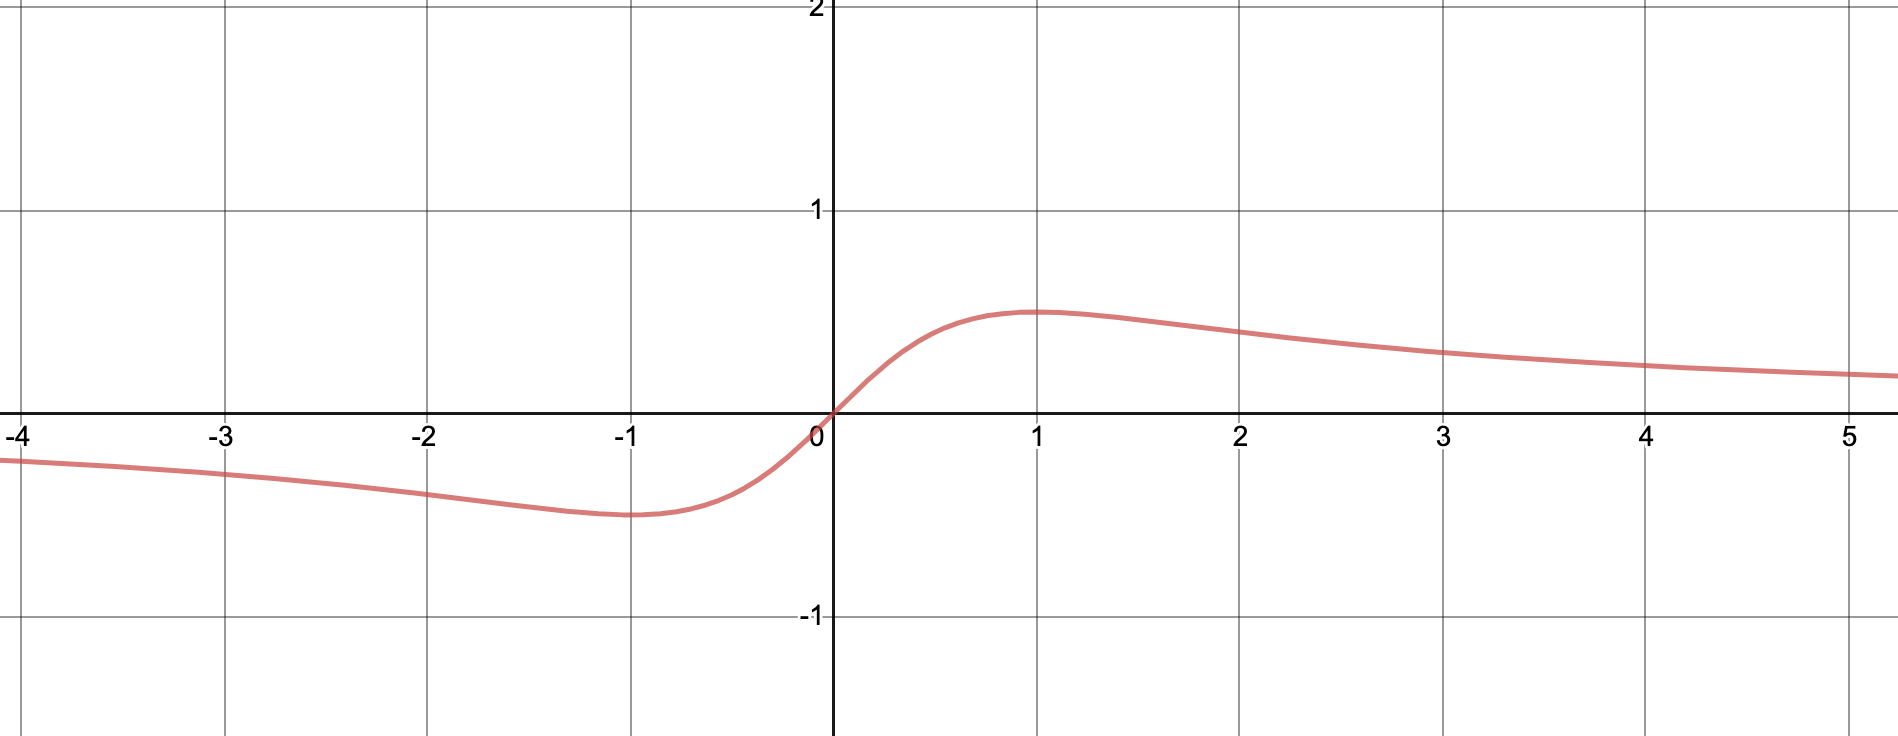
\includegraphics[scale=0.5]{pics/new5}\\

Now let's apply Newton's method with two initial approximations $x_0 = 2$ and $x_0=\frac{1}{\sqrt{3}}$:
\end{examplebox}

\newpage
\section{Quadratic Model}
\marginnote{
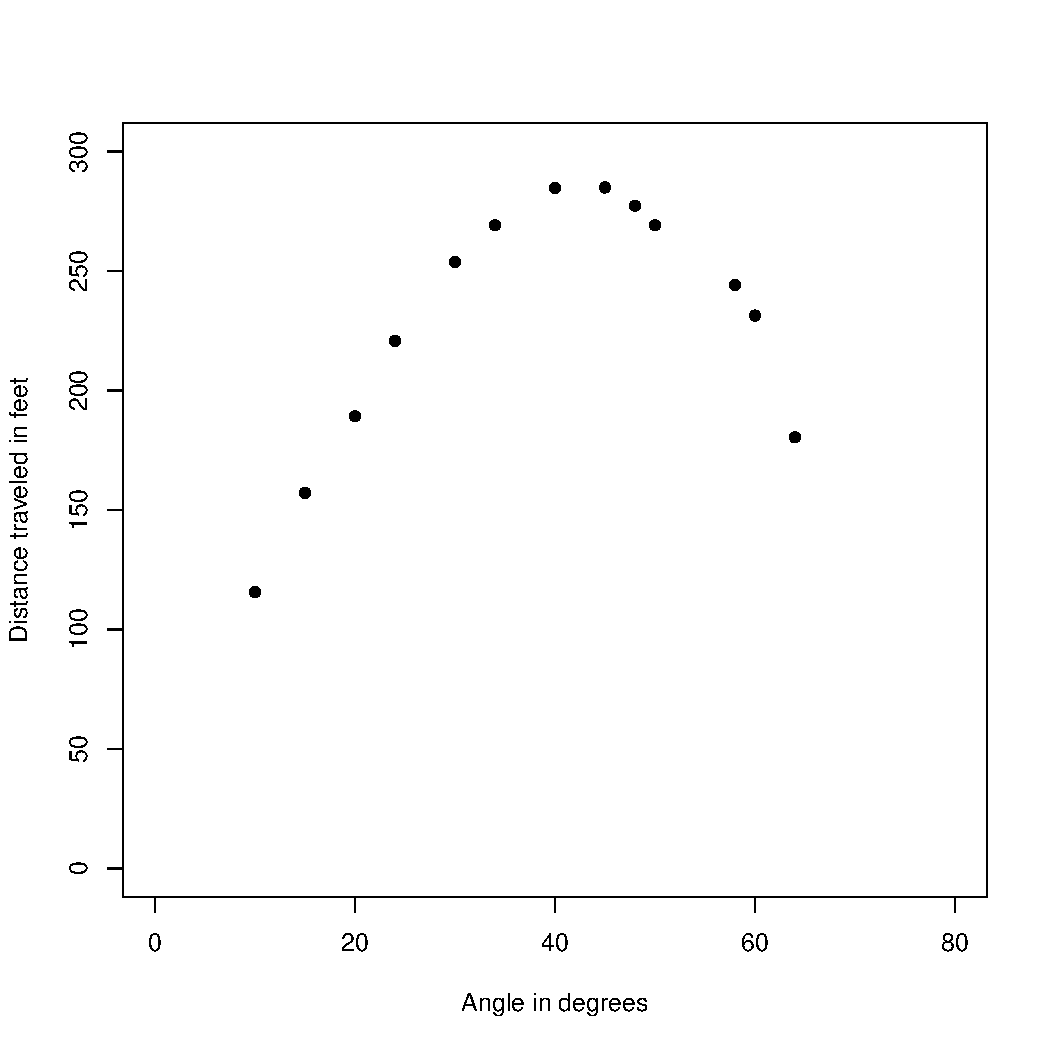
\includegraphics{pics/scatterplot}
}
\begin{examplebox}{}

\emph{Problem Statement:}

We aim to model the distance a baseball travels as a function of the hitting angle using a quadratic function.

\emph{Model Specification:}

Let
\begin{itemize}
	\item $Y_{i}$ denote the random variable of the distance traveled by the baseball (in feet) for the $i$-th observation. The actual observed data of $Y_{i}$ is denoted by $y_{i}$.
	\item $X_{i}$ denote the random variable of the hitting angle (in degrees) for the $i$-th observation. The actual observed data of $X_{i}$ is denoted by $x_{i}$
\end{itemize}

The relationship between the distance and the hitting angle is modeled as:
$Y_{i} = \alpha + \beta X_{i} + \gamma X_{i}^{2 } + \epsilon_{i}$

where:
\begin{itemize}
	\item $\alpha,\beta,\gamma$ are the parameters to be estimated.
	\item $\epsilon_{i}$ represents the error term, assumed to be normally distributed with mean $0$ and variance $\sigma^{2}$, i.e. $\epsilon_{i} \sim N(0, \sigma^{2})$.
\end{itemize}

\emph{Objective:}

Given a dataset $\{(y_{i}, x_{i})\}^{n }_{i=1}$, our goal is to estimate the parameters $\alpha, \beta, \gamma,$ and $\sigma^{2}$.

\end{examplebox}

Because of $Y_{i} \sim N(\alpha + \beta X_{i} + \gamma X_{i}^{2}, \sigma^{2})$,

The probability density function of $Y_{i } = y_{i}$ is:

\[
P(Y_{i } = y_{i }|x_{i}, \alpha, \beta, \gamma, \sigma^{2}) = \frac{1 }{\sigma\sqrt{2 \pi }} e^{- \frac{1 }{2 \sigma^{2 }}(y_{i }-\alpha-\beta x_{i } - \gamma x_{i }^{2})^{2}}
\]

The likelihood function of $(\alpha,\beta,\gamma,\sigma^{2})$ is:

\begin{align*}
	L(\alpha,\beta,\gamma,\sigma^{2}|\{(y_{i}, x_{i})\}^{n }_{i=1}) &= \prod^{n }_{i=1 }P(Y_{i } = y_{i }|x_{i}, \alpha, \beta, \gamma, \sigma^{2}) \\
	&=\left(\frac{1 }{\sigma\sqrt{2 \pi }}\right)^{n} e^{- \frac{1 }{2 \sigma^{2 }} \sum^{n }_{i=1}(y_{i }-\alpha-\beta x_{i } - \gamma x_{i }^{2})^{2}}\\
	&=(2\pi)^{-\frac{n }{2 }} (\sigma^{2 })^{-\frac{n}{2}} e^{-\frac{1}{2 \sigma^{2}} \sum^{n }_{i=1}(y_{i }-\alpha-\beta x_{i } - \gamma x_{i }^{2})^{2}}\\
\end{align*}

Taking the log on both sides of the equation yields the following log likelihood function:

\begin{equation}
l(\alpha,\beta,\gamma,\sigma^{2}) = \ln L(\alpha,\beta,\gamma,\sigma^{2}) = -\frac{n}{2} \ln(2\pi) - \frac{n }{2 }\ln(\sigma^{2}) - \frac{1 }{2 \sigma^{2}}\sum^{n }_{i=1 }(y_{i }-\alpha-\beta x_{i } - \gamma x_{i }^{2})
	\label{eq:loglikelihood}
\end{equation}


We want to find the value of $(\alpha,\beta,\gamma,\sigma^{2})$ such that equation~\ref{eq:loglikelihood} gets its maximum.

Consider the gradient of $l(\alpha,\beta,\gamma,\sigma^{2})$:

\[
	\nabla l(\boldsymbol{\Theta}) = \begin{pmatrix}
		\frac{\partial l}{\partial \alpha}\\
		\frac{\partial l}{\partial \beta}\\
		\frac{\partial l}{\partial \gamma}\\
		\frac{\partial l}{\partial \sigma^{2}}
	\end{pmatrix}
	,\qquad \text{ where }\boldsymbol{\Theta } = \begin{pmatrix}
		\alpha\\
		\beta\\
		\gamma\\
		\sigma^{2}
\end{pmatrix}
\]

\begin{align*}
	\frac{\partial l}{\partial \alpha} &= -\frac{1 }{2 \sigma^{2 }} \sum^{n }_{i=1 }2(y_{i }-\alpha-\beta x_{i }-\gamma x_{i }^{2}) (-1)\\
	&= \frac{1 }{\sigma^{2 }} \sum^{n }_{i=1 }(y_{i }-\alpha-\beta x_{i }-\gamma x_{i }^{2})\\
	\frac{\partial l}{\partial \beta} &= -\frac{1}{2\sigma^{2}} \sum^{n }_{i=1 }2(y_{i }-\alpha-\beta x_{i }-\gamma x_{i }^{2 })(-x_{i})\\
&= \frac{1}{\sigma^{2}} \sum^{n }_{i=1 }(x_{i})(y_{i }-\alpha-\beta x_{i }-\gamma x_{i }^{2 })\\
&= \frac{1}{\sigma^{2}}\left( \sum^{n }_{i=1 }x_{i }y_{i } -\alpha\sum^{n }_{i=1 }x_{i} -\beta \sum^{n }_{i=1 }x_{i }^{2} -\gamma \sum^{n }_{i=1}x_{i }^{3}\right)\\
	\frac{\partial l}{\partial \gamma} &= -\frac{1 }{2 \sigma^{2 }} \sum^{n }_{i=1 }2(y_{i }-\alpha-\beta-\gamma x_{i }^{2})(-x_{i }^{2})\\
 &= \frac{1 }{\sigma^{2 }} \sum^{n }_{i=1 }(x_{i }^{2})(y_{i }-\alpha-\beta-\gamma x_{i }^{2})\\
 &= \frac{1 }{\sigma^{2 }} \left(\sum^{n }_{i=1 }x_{i }^{2}y_{i} -\alpha \sum^{n }_{i=1 }x_{i }^{2} - \beta \sum^{n }_{i=1 }x_{i }^{3} - \gamma \sum^{n }_{i=1 }x_{i }^{4} \right)\\
	\frac{\partial l}{\partial \sigma^{2}} &= - \frac{n }{2 \sigma^{2 }} - \frac{(-1)(\sigma^{2 })^{-2} }{2 } \sum^{n }_{i=1 }(y_{i }- \alpha - \beta x_{i }- \gamma x_{i }^{2 })^{2}\\
&= - \frac{n }{2 \sigma^{2 }} + \frac{1}{2\sigma^{4}} \sum^{n }_{i=1 }(y_{i }- \alpha - \beta x_{i }- \gamma x_{i }^{2 })^{2}\\
\end{align*}

The Hessian matrix of the likelihood function is:

\[
	\nabla^{2}l(\boldsymbol{\Theta}) = \begin{bmatrix}
		\frac{\partial^{2}l}{\partial \alpha^{2}} &
		\frac{\partial^{2}l}{\partial \alpha \partial \beta} &
		\frac{\partial^{2}l}{\partial \alpha \partial \gamma} &
		\frac{\partial^{2}l}{\partial \alpha \partial \sigma^{2}} \\
		\frac{\partial^{2}l}{\partial \beta \partial \alpha} &
		\frac{\partial^{2}l}{\partial \beta^{2} } &
		\frac{\partial^{2}l}{\partial \beta \partial \gamma} &
		\frac{\partial^{2}l}{\partial \beta \partial \sigma^{2}} \\
		\frac{\partial^{2}l}{\partial \gamma \partial \alpha} &
		\frac{\partial^{2}l}{\partial \gamma \partial \beta} &
		\frac{\partial^{2}l}{\partial \gamma^{2} } &
		\frac{\partial^{2}l}{\partial \gamma \partial \sigma^{2}} \\
		\frac{\partial^{2}l}{\partial \sigma^{2} \partial \alpha} &
		\frac{\partial^{2}l}{\partial \sigma^{2} \partial \beta} &
		\frac{\partial^{2}l}{\partial \sigma^{2} \partial \gamma} &
		\frac{\partial^{2}l}{(\partial \sigma^{2})^{2} }
	\end{bmatrix}
\]

Calculate the second-order partial derivatives yields:

\begin{align*}
	&\nabla^{2}l(\boldsymbol{\Theta}) \\
	=& \begin{bmatrix}
		- \frac{n }{\sigma^{2}}&
		- \frac{\sum x_{i }}{\sigma^{2}}&
		- \frac{\sum x_{i }^{2}}{\sigma^{2}}&
		- \frac{\left(\sum y_{i} -n \alpha -\beta \sum x_{i } - \gamma \sum x_{i }^{2}\right)}{\sigma^{4}} \\
		- \frac{\sum x_{i }}{\sigma^{2}}&
		- \frac{\sum x_{i }^{2}}{\sigma^{2}}&
		- \frac{\sum x^{3 }_{i }}{\sigma^{2}} &
		- \frac{\left( \sum x_{i }y_{i } - \alpha \sum x_{i } - \beta \sigma x_{i}^2 - \gamma \sigma x_{i }^{3}\right)}{\sigma^{4}} \\
		- \frac{\sum x_{i }^{2}}{\sigma^{2}} &
		- \frac{\sum x^{3 }_{i }}{\sigma^{2}} &
		- \frac{\sum x_{i}^{4}}{\sigma^{2}} &
		- \frac{\left(\sum x_{i}^{2}y_{i} - \alpha \sum x_{i}^{2} - \beta \sum x_{i}^{3} - \gamma \sum x_{i}^{4}\right)}{\sigma^{4}} \\
		- \frac{\left(\sum y_{i} -n \alpha -\beta \sum x_{i } - \gamma \sum x_{i }^{2}\right)}{\sigma^{4}} &
		- \frac{\left( \sum x_{i }y_{i } - \alpha \sum x_{i } - \beta \sigma x_{i}^2 - \gamma \sigma x_{i }^{3}\right)}{\sigma^{4}} &
		- \frac{\left(\sum x_{i}^{2}y_{i} - \alpha \sum x_{i}^{2} - \beta \sum x_{i}^{3} - \gamma \sum x_{i}^{4}\right)}{\sigma^{4}} &
		\frac{\partial^{2}l}{(\partial \sigma^{2})^{2} }
	\end{bmatrix}
\end{align*}

The last element

\begin{align*}
\frac{\partial^{2}l}{(\partial \sigma^{2})^{2}}
&= -\frac{n }{2 }(-1)(\sigma^{2 })^{-2} + \frac{1 }{2 } (-2) (\sigma^{3})^{-3} \sum^{n }_{i=1 }(y_{i} - \alpha -\beta x_{i } - \gamma x_{i }^{2})^{2}\\
&= \frac{n }{2 \sigma^{4}} - \frac{\sum^{n }_{i=1 } (y_{i }-\alpha - \beta x_{i } - \gamma x_{i }^{2})^{2}}{\sigma^{6}}
\end{align*}

Hence, using the Newton-Raphson method, the iteration formula for $\boldsymbol{\Theta}$ is:

\begin{equation}
	\boldsymbol{\Theta}^{\text{new}} = \boldsymbol{\Theta}^{\text{old}} - \left(\nabla^{2}l(\boldsymbol{\Theta}^{\text{old}})\right)^{-1}\left(\nabla l(\boldsymbol{\Theta}^{\text{old}})\right)
	\label{eq:iterTheta}
\end{equation}
